\documentclass[12pt]{article}
\usepackage[T1]{fontenc}
\usepackage{amsmath}
\usepackage{amssymb}
\usepackage{amssymb}
\usepackage{color}
\usepackage[utf8]{inputenc}
\usepackage{tikz}
\usetikzlibrary{arrows.meta,backgrounds,calc,fit,positioning,scopes,shadows}
\def\tikzsavelastnodename#1{\let#1=\tikz@last@fig@name}

\begin{document}

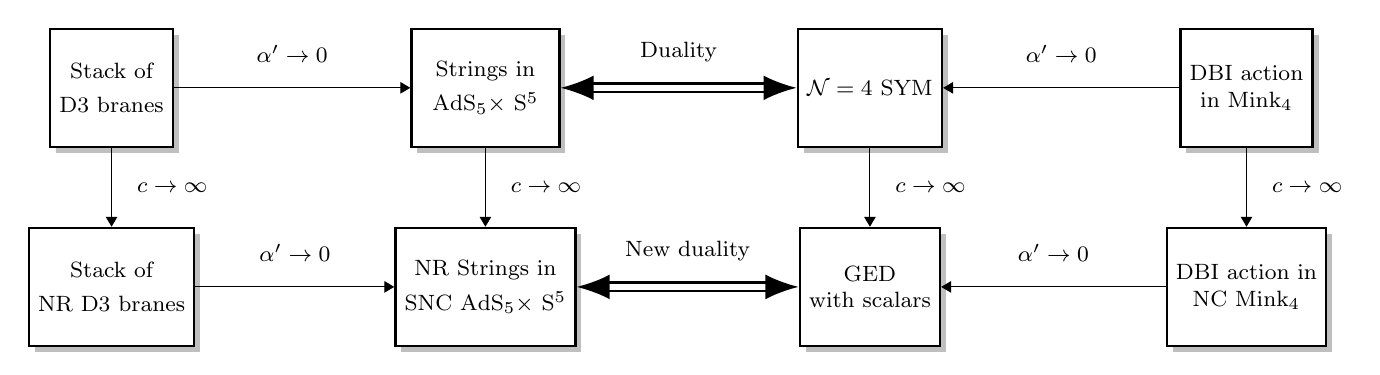
\begin{tikzpicture}[> = {Triangle[]},atomic/.style = {draw, thick, fill=white, font=\footnotesize,minimum size=1.5cm, drop shadow,append after command= {\pgfextra{\tikzsavelastnodename\tikzsavednodename}},#1}]
%---
\node[atomic,align=center]                         (D3)     {Stack of \\[1mm]
D3 branes};

\node[atomic,align=center,right=3cm of D3]                         (NHL)     {Strings in \\[1mm]
 \, AdS$_5 \times$ S$^5$ \, };

\node[atomic,align=center,below=1cm of D3]                         (NRD3)     {Stack of \\[1mm]
NR D3 branes};

\node[atomic,align=center,below=1cm of NHL]                         (NRNHL)     {NR Strings in \\[1mm] 
SNC AdS$_5 \times$ S$^5$};


\node[atomic,align=center,right=3cm of NHL]                         (N4SYM)     {$\mathcal{N}=4$ SYM};


\node[atomic,align=center,below=1cm of N4SYM]                         (NRN4SYM)     {GED\\
with scalars};


\node[atomic,align=center,right=3cm of N4SYM]                         (DBI)     {DBI action \\
in Mink$_4$};


\node[atomic,align=center,below=1cm of DBI]                         (NRDBI)     {DBI action in\\
NC Mink$_4$};


\draw[->] (D3) -- node [font=\footnotesize,midway,above=0.2cm,align=center ]{$\alpha ' \rightarrow 0$} (NHL);
\draw[->] (NHL) -- node [font=\footnotesize,midway,right=0.2cm,align=center ]{$c\rightarrow \infty$} (NRNHL);
\draw[->] (NRD3) -- node [font=\footnotesize,midway,above=0.2cm,align=center ]{$\alpha ' \rightarrow 0$} (NRNHL);
\draw[->] (D3) -- node [font=\footnotesize,midway,right=0.2cm,align=center ]{$c\rightarrow \infty$} (NRD3);
\draw [line width=1pt, double distance=2pt,
arrows = {Latex[length=0pt 3 0]-Latex[length=0pt 3 0]}]  (NHL) -- node [font=\footnotesize,midway,above=0.2cm,align=center ]{Duality} (N4SYM);
\draw [line width=1pt, double distance=2pt,
arrows = {Latex[length=0pt 3 0]-Latex[length=0pt 3 0]}] (NRNHL) -- node [font=\footnotesize,midway,above=0.2cm,align=center ]{New duality} (NRN4SYM);
\draw[->] (N4SYM) -- node [font=\footnotesize,midway,right=0.2cm,align=center ]{$c\rightarrow \infty$} (NRN4SYM);
\draw[<-] (N4SYM) -- node [font=\footnotesize,midway,above=0.2cm,align=center ]{$\alpha ' \rightarrow 0$} (DBI);
\draw[<-] (NRN4SYM) -- node [font=\footnotesize,midway,above=0.2cm,align=center ]{$\alpha ' \rightarrow 0$} (NRDBI);
\draw[->] (DBI) -- node [font=\footnotesize,midway,right=0.2cm,align=center ]{$c\rightarrow \infty$} (NRDBI);
\end{tikzpicture}

\end{document}